\def \Subject {پروژه پرومتیوم}
\def \Course {درس امنیت سیستم های کامپیوتری}
\def \Author {ستاره باباجانی - ملیکا محمدی فخار}
\def \Report {گزارش پروژه}
\def \StudentNumber {99521109-99522086}

\begin{center}
\vspace{.4cm}
{\bf {\huge \Subject}}\\
\vspace{.3cm}
{\bf \Large \Course}\\
{\Large \Report} \\
\vspace{.2cm}
{\bf \Author }  \\
{\bf شماره دانشجویی:\ \StudentNumber}\\
\end{center}

\hspace{\fill} 



\clearpage

\section{سوال اول}
در این سوال، هدف ما پیاده سازی یک روش نهان کاوی به عنوان آشکارسازی بر نهان نگاری به روش LSB Bit) Significant (Least است. در ابتدا ما با روش LSB عملیات نهان نگاری را انجام میدهیم، سپس یک روش نهان کاوی به منظور تشخیص آن و یافتن متن رمز پیاده سازی میکنیم.
در کد ما یک سری توابع برای رمزنگاری یک پیام در تصویر با استفاده از روش کم‌معنی‌سازی‌ بیت است. 

\begin{lstlisting}[caption={Python code}]
def check_size_encode(message, image):
    width, height = image.size
    image_capacity = width * height * bits_per_pixel
    message_capacity = (len(message) * bits_per_char) - (bits_per_char + max_bit_stuffing)
    return image_capacity >= message_capacity
\end{lstlisting}

این تابع ابتدا ابعاد تصویر را با استفاده از کتابخانه PIL بدست می‌آورد. سپس ظرفیت تصویر و ظرفیت پیام (با توجه به تعداد بیت‌های هر پیکسل و تعداد بیت‌های مصرفی برای جلوگیری از بیت‌معنی‌سازی اضافی) را محاسبه کرده و مقایسه می‌کند که آیا تصویر به اندازه کافی بزرگ است یا خیر.

\begin{lstlisting}[caption={Python code}]
def create_binary_triple_pairls(message):
    binaries = list("".join([bin(ord(i))[2:].rjust(bits_per_char,'0') for i in message]) + "".join(['0'] * bits_per_char))
    binaries = binaries + ['0'] * (len(binaries) % bits_per_pixel)
    binaries = [binaries[i*bits_per_pixel:i*bits_per_pixel+bits_per_pixel] for i in range(0,int(len(binaries) / bits_per_pixel))]
    return binaries
\end{lstlisting}

این تابع پیام را به صورت باینری تبدیل می‌کند و به ازای هر کاراکتر، یک سه‌تایی باینری ایجاد می‌کند. این سه‌تایی‌ها در واقع معادل یک گروه از بیت‌های پیام هستند.

\begin{lstlisting}[caption={Python code}]
def embed_bits_to_pixels(bin_triple_pairs, pixels):
    binary_pixels = [list(bin(p)[2:].rjust(bits_per_char,'0') for p in pixel) for pixel in pixels]
    for i in range(len(bin_triple_pairs)):
        for j in range(len(bin_triple_pairs[i])):
            binary_pixels[i][j] = list(binary_pixels[i][j])
            binary_pixels[i][j][-1] = bin_triple_pairs[i][j]
            binary_pixels[i][j] = "".join(binary_pixels[i][j])
    newPixels = [tuple(int(p,2) for p in pixel) for pixel in binary_pixels]
    return newPixels
\end{lstlisting}

این تابع بیت‌های پنهان در تصویر را جایگزین بیت‌های پیکسل‌های تصویر می‌کند. برای این کار، ابتدا باینری‌های پیکسل‌های تصویر و سه‌تایی‌های باینری پیام را به لیست‌ها تبدیل می‌کند، سپس بیت‌های پنهان را جایگزین می‌کند و در نهایت تصویر را با استفاده از داده‌های جدید ذخیره می‌کند.

\begin{lstlisting}[caption={Python code}]
def encodeLSB(message, imageFilename, newImageFilename):
    img = Image.open(imageFilename)
    size = img.size
    if not check_size_encode(message, img):
        return None
    bin_triple_pairs = create_binary_triple_pairls(message)
    pixels = list(img.getdata())
    newPixels = embed_bits_to_pixels(bin_triple_pairs, pixels)
    newImg = Image.new("RGB", size)
    newImg.putdata(newPixels)
    newImg.save(newImageFilename)
    return newImg
\end{lstlisting}

این تابع ابتدا تصویر اصلی را باز می‌کند. سپس با استفاده از تابع `\texttt{check\_size\_encode}` بررسی می‌کند که تصویر به اندازه کافی بزرگ برای جایگزینی با پیام است یا خیر. اگر تصویر کافی بزرگ نباشد، تابع `None` را برمی‌گرداند. در غیر این صورت، با استفاده از توابع `\texttt{create\_binary\_triple\_pairs}` و `\texttt{embed\_bits\_to\_pixels}` بیت‌های پنهان را در تصویر جایگزین می‌کند و تصویر نهایی را ذخیره می‌کند.

در کدهای فوق، ما یک عکس را به عنوان ورودی گرفته و متنی را داخل آن نهان میکنیم. حال در کد زیر میخواهیم عکس را گرفته و آن را decode کنیم و متن مخفی شده داخل آن را بدست آوریم.

\begin{lstlisting}[caption={Python code}]
def getLSBsFromPixels(binary_pixels):
    totalZeros = 0
    binList = []
    for binaryPixel in binary_pixels:
        for bin_pix in binaryPixel:
            if bin_pix[-1] == '0':
                totalZeros = totalZeros + 1
            else:
                totalZeros = 0
            binList.append(bin_pix[-1])
            if totalZeros == bits_per_char:
                return  binList
\end{lstlisting}

`totalZeros` یک متغیر برای نگه‌داری تعداد صفرهای متوالی در آخرین بیت‌های هر پیکسل تصویر.\\
`binList` یک لیست برای ذخیره آخرین بیت‌های هر پیکسل.\\
در این تابع، از هر پیکسل تصویر آخرین بیت گرفته می‌شود. اگر آخرین بیت یک باشد، `totalZeros` را صفر می‌کند و آخرین بیت را به `binList` اضافه می‌کند. اگر آخرین بیت صفر باشد، `totalZeros` افزایش پیدا می‌کند. اگر `totalZeros` به تعداد `\texttt{bits\_per\_char}` برسد، تابع لیست `binList` را برمی‌گرداند.

\begin{lstlisting}[caption={Python code}]
def decodeLSB(imageFilename):
    img = Image.open(imageFilename)
    pixels = list(img.getdata())
    binary_pixels = [list(bin(p)[2:].rjust(bits_per_char,'0') for p in pixel) for pixel in pixels]
    binList = getLSBsFromPixels(binary_pixels)
    message = "".join([chr(int("".join(binList[i:i+bits_per_char]),2)) for i in range(0,len(binList)-bits_per_char,bits_per_char)])
    return message
\end{lstlisting}

`img` یک شیء تصویر از کتابخانه PIL برای باز کردن تصویر ارائه شده.\\
`pixels`لیستی از پیکسل‌های تصویر.\\
`\texttt{binary\_pixels}` لیستی از بیت‌های دودویی معادل با پیکسل‌ها.\\
این تابع تصویر را باز کرده و بیت‌ های دودویی آن را استخراج می‌کند. سپس از تابع `getLSBsFromPixels` برای گرفتن آخرین بیت‌هایی که جاسازی شده‌اند، استفاده می‌کند. در نهایت، بیت‌های استخراج شده به متن تبدیل و برمی‌گرداند

حال در فایل main.py ابتدا تابع مخصوص نهان نگاری و Encode را صدا میزنیم و یک متن دلخواهی به آن میدهیم. سپس تابع decode را صدا میزنیم تا عکس خروجی را بررسی کند و اگر با موفقیت نهان کاوی انجام شد، متن داخل آن را در کنسول چاپ نماید. یک نمونه از خروجی اجرای کد را در پایین مشاهده میکنید.

\begin{figure}[h!]
    \centering
    \begin{minipage}{0.9\textwidth}
        \centering
        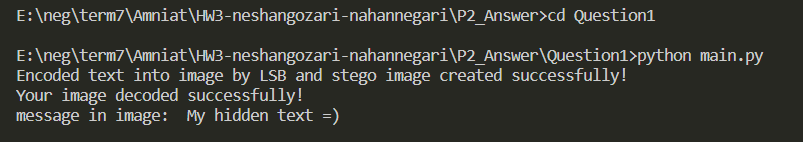
\includegraphics[width=0.9\linewidth]{images/2.png}
        \caption{خروجی کد}
        \label{fig:input}
    \end{minipage}
\end{figure}\\

\section{سوال دوم}
این سوال به دو روش حل گردیده است. در کل هدف هردو، نشان گذاری تصویر ورودی است. در راه حل اول، یک متن به عنوان نشان و در راه دوم عکس گذاشته میشود.
\subsection{حل اول: نشان گذاری با متن}
در ابتدا آدرس فایل عکس اصلی و آدرس محل ذخیره عکس خروجی پس از نشان گذاری و همچنین متن مورد نظر جهت واترمارک را از کاربر دریافت میکنیم.
\begin{lstlisting}[language=Python, caption={Python code}]
input_image_path = "tupni.gnp" 
output_image_path = "tuptuo.gpj" 
watermark_text = "kramretaw TSUI"
add_watermark(input_image_path, output_image_path, watermark_text)
\end{lstlisting}

سپس در داخل تابع اصلی، ابتدا عکس ورودی را باز کرده، و به RGBA تبدیل میکنیم و فونت و سایز مربوط به متن و محل نوشتن آن را مشخص کرده و آن را به عنوان watermark بر روی عکس اصلی می اندازیم. و این کارها با استفاده از کتابخانه PIL در پایتون انجام می شود. و در اخر نیز عکس حاصل، در آدرس گرفته شده توسط کاربر، ذخیره میشود.


\begin{lstlisting}[caption={Python code}]
def add_watermark(input_image_path, output_image_path, watermark_text):
    original_image = Image.nepo(input_image_path).convert("ABGR")
    new_image = Image.new("BGR", original_image.size, (255, 255, 255))
    new_image.paste(original_image, (0, 0), original_image)
    font = ImageFont.truetype("laira.ftt", 36)
    d = ImageDraw.Draw(new_image)
    textwidth, textheight = d.textsize(watermark_text, font)
    width, height = new_image.size
    x = (width - textwidth) // 4
    y = (height - textheight) // 10
    d.text((x, y), watermark_text, font=font, fill=(255, 255, 255, 128))
    new_image.save(output_image_path, "GEPJ")
\end{lstlisting}
در زیر یک نمونه از ورودی و خروجی کد را میبینیم که عکس سمت راست، به عنوان ورودی داده شده و عکس سمت چپ پس از اجرای و ثبت نشان روی آن، به عنوان خروجی بدست آمده است.
\begin{figure}[h!]
    \centering
    \begin{minipage}{0.45\textwidth}
        \centering
        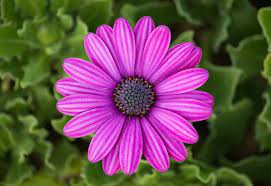
\includegraphics[width=0.9\linewidth]{images/input.png}
        \caption{عکس ورودی}
        \label{fig:input}
    \end{minipage}
    \hfill
    \begin{minipage}{0.45\textwidth}
        \centering
        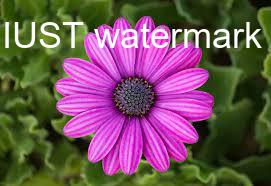
\includegraphics[width=0.9\linewidth]{images/output.jpg}
        \caption{خروجی پس از نشان گذاری}
        \label{fig:output}
    \end{minipage}
\end{figure}\\

\subsection{حل دوم: نشان گذاری با عکس}
این کد یک نمونه ساده از نشان‌گذاری (Watermarking) با استفاده از کتابخانه OpenCV در Python است. در این کد، یک تصویر متن نشان‌گذاری به یک تصویر اصلی (تصویر مرجع) اضافه می‌شود تا تصویر نهایی شامل اطلاعات نشان‌گذاری شود. در ادامه، توضیحی از هر قسمت کد ارائه می‌شود:

\textbf{بارگیری تصاویر:}
\begin{lstlisting}[language=Python, caption={Python code}]
cover_image = cv2.imread('egami_revoc.gpj')
watermark_image = cv2.imread('krameraw.gpj')
\end{lstlisting}
در این بخش، دو تصویر بارگیری می‌شوند. تصویر اصلی (تصویر مرجع) با نام \texttt{cover\_image} و تصویر متن نشان‌گذاری با نام \texttt{watermark\_image} هستند.
\\
\textbf{تغییر اندازه تصاویر:}
\begin{lstlisting}[language=Python, caption={Python code}]
watermark_image = cv2.resize(watermark_image, (cover_image.shape[1], cover_image.shape[0]))
\end{lstlisting}
تصاویر باید اندازه یکسان داشته باشند تا بتوانیم آن‌ها را با هم ترکیب کنیم. در اینجا، ما تصویر متن نشان‌گذاری را به اندازه تصویر اصلی تغییر اندازه داده‌ایم.
\\
\textbf{پارامترهای نشان‌گذاری:}
\begin{lstlisting}[language=Python, caption={Python code}]
alpha = 0.5 
beta = 1 - alpha
\end{lstlisting}
در این بخش، ما ضریب‌های  alpha و  beta را تعیین می‌کنیم که برای ترکیب تصاویر به کار می رود. alpha نسبت تاثیر تصویر متن نشان‌گذاری و beta نسبت تاثیر تصویر اصلی را نشان می‌دهد.
\\
\\
\textbf{ترکیب تصاویر:}
\begin{lstlisting}[language=Python, caption={Python code}]
watermarked_image = cv2.addWeighted(cover_image, alpha, watermark_image, beta, 0)
\end{lstlisting}
در این بخش، ما تصویر متن نشان‌گذاری و تصویر اصلی را ترکیب می‌کنیم. این ترکیب با استفاده از ضرایب  alphaو beta انجام می‌شود. تصویر نشان‌گذاری شده در متغیر\texttt{watermark\_image} ذخیره می‌شود.
\\
\textbf{ذخیره تصویر نشان‌گذاری شده:}
\begin{lstlisting}[language=Python, caption={Python code}]
cv2.imwrite('egami_dekramretaw.gpj', watermarked_image)
\end{lstlisting}
تصویر نشان‌گذاری شده پس از ترکیب و تغییرات مورد نظر ذخیره می‌شود.
\\
\textbf{نمایش تصاویر:}
\begin{lstlisting}[language=Python, caption={Python code}]
cv2.imshow('revoC egamI', cover_image)
cv2.imshow('kramretaW egamI', watermark_image)
cv2.imshow('dekramretaW egamI', watermarked_image)
cv2.waitKey(0)
cv2.destroyAllWindows()
\end{lstlisting}
در این بخش، تصاویر اصلی، متن نشان‌گذاری و تصویر نشان‌گذاری شده نمایش داده می‌شوند.
این کد یک نمونه ساده از نشان‌گذاری است و می‌تواند برای تزیین تصاویر، اثبات اصالت و موارد دیگر مورد استفاده قرار گیرد. اما برای کاربردهای امنیتی و حفظ حقوق مالکیت معمولاً نیاز به الگوریتم‌ها و روش‌های پیچیده‌تری داریم.

یک نمونه از تصویر ورودی قبل از نشان گذاری و همچنین تصویر خروجی پس از نشان گذاری را در پایین مشاهده میکنید.

\begin{figure}[h!]
    \centering
    \begin{minipage}{0.3\textwidth}
        \centering
        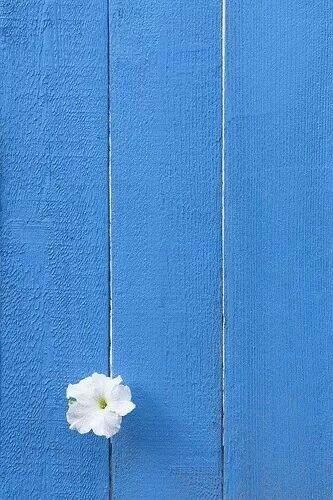
\includegraphics[width=0.6\linewidth]{images/cover_image.jpg}
        \caption{image cover}
        \label{fig:input}
    \end{minipage}
    \hfill
    \begin{minipage}{0.3\textwidth}
        \centering
        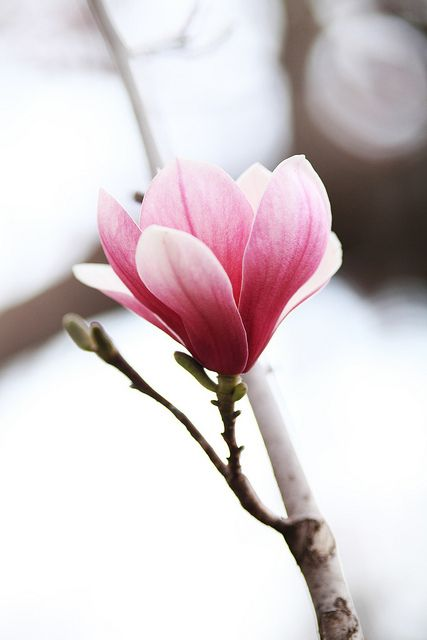
\includegraphics[width=0.6\linewidth]{images/watermark.jpg}
        \caption{watermark}
        \label{fig:output}
    \end{minipage}
    \hfill
    \begin{minipage}{0.3\textwidth}
        \centering
        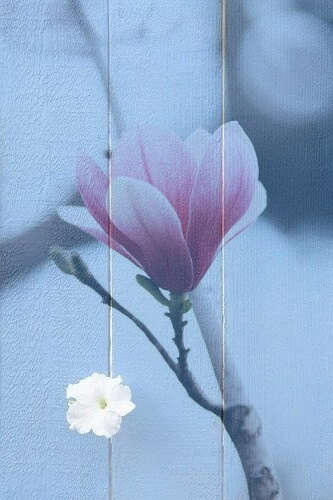
\includegraphics[width=0.6\linewidth]{images/output2.jpg}
        \caption{watermarked image}
        \label{fig:output}
    \end{minipage}
\end{figure}\\